\section{Semaine 4 : 27/02/2023 - 03/03/2023}
\graphicspath{{semaines/semaine_4/images/}}

\begin{abstract}
	On cherche à comprendre les problèmes d'interpolation de phi dans le cadre de la correction sur la solution exacte du problème de poisson avec condition de dirichlet homogène. Après la réunion du 28/02 avec Emmanuel et Vanessa, les points suivants sont à traiter :
	\begin{enumerate}[label=\textbullet]
		\item tester avec solution analytique + perturbation !
		\item enlever les termes de stabilisation afin de voir si le problème est dans la dérivée seconde de phi
		\item visualiser le $\phi$ et le $\phi'$ EF et le comparer au $\phi$ et $\phi'$ analytique
		\item comprendre le problème du extrapolate
	\end{enumerate}
	Après la réception d'un ordinateur, on a passé la moitié de la semaine à essayer d'installer ce dont on avait besoin. En fin de semaine, les installations ont enfin été faite et je peux maintenant générer des données et entraîner le modèle sur ce nouveau PC.
\end{abstract}

\subsection{Génération des données}

On considère toujours $\Omega$ le cercle de rayon $\sqrt{2}/4$ et de centre $(0.5,0.5)$ avec $\Phi(x,y)=-1/8+(x-1/2)^2+(y-1/2)^2$ et le domaine fictif $O=(0,1)^2$.

On souhaite résoudre 
\begin{equation*}
	\begin{cases}
		-\Delta u &= f\,, \quad \text{dans $\Omega$}\,, \\
		u &= 0\,, \quad \text{sur $\Gamma$}\,, \\
	\end{cases}
\end{equation*}

Notre solution analytique est
$$u_{ex}(x,y) = \frac{1}{\sin\left(k_1\frac{\pi}{2}\right)}\times\sin\left(k_1\frac{\pi}{2}\left(\frac{4}{\sqrt{2}}\right)^2\left((x-0.5)^2+(y-0.5)^2\right)\right)\times\cos\left(\frac{\pi}{2}\left(\frac{4}{\sqrt{2}}\right)^2\left((x-0.5)^2+(y-0.5)^2\right)\right)\,, $$ 

avec $k_1 \sim \mathcal{U}([0.1,0.5])$.

\subsection{Correction}

On cherche à comprendre les problèmes d'interpolation de phi dans le cadre de la correction sur la solution exacte du problème de poisson avec condition de Dirichlet homogène (\href{https://colab.research.google.com/drive/17S0TrfstBv8vk6KR3uAy8gbeOcSkWPsY#scrollTo=7i8HL9-JKfEj}{"tests\_interpolation"}). On va effectuer plusieurs tests :

\subsubsection*{Solution analytique + Perturbation.}

Pour simuler la solution fournit par le FNO on va considérer comme nouvelle level-set notre solution analytique plus une petite perturbation. La perturbation choisie est définie par :
$$P(x,y)=\epsilon\times\sin(k_1(x+y))\times\cos(4\pi((x-0.5)^2+(y-0.5)^2))$$
On a alors
$$\Phi(x,y)=u_{ex}(x,y)+P(x,y)$$
En prenant $\epsilon=1$, on a :

\begin{minipage}{\linewidth}
	\centering
	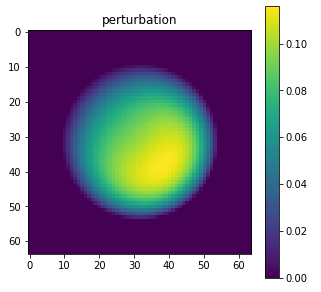
\includegraphics[width=0.3\linewidth]{perturbation.png}
\end{minipage}

On obtient en normes $L_2$ les différentes erreurs en fonction de $\epsilon=1e-k$ entre la solution initiale fournit $\Phi$ et le solution après correction $\Phi C$ : 

\begin{minipage}{\linewidth}
	\centering
	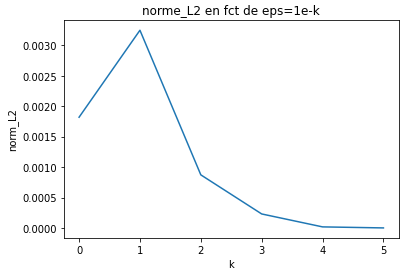
\includegraphics[width=0.45\linewidth]{erreurs_perturb.png}
\end{minipage}

Il semblerait que plus la perturbation est petite et plus l'erreur est petite. De plus, $C$ est de plus en plus proche de 1 :

\begin{minipage}{\linewidth}
	\centering
	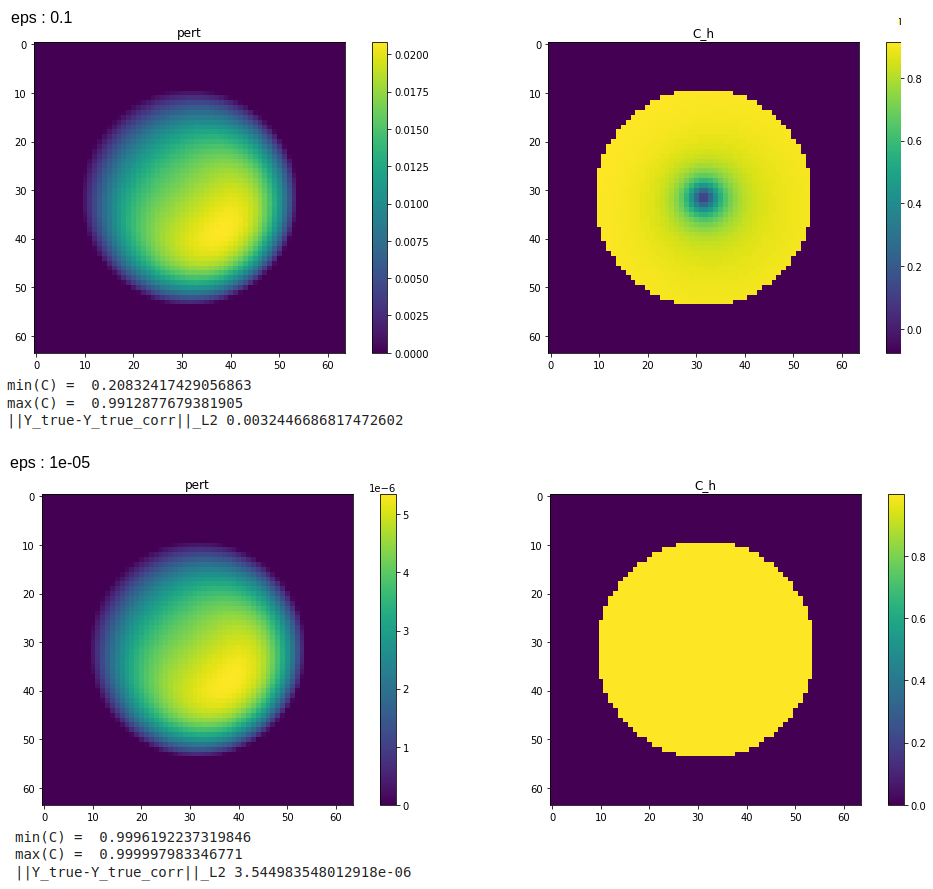
\includegraphics[width=0.55\linewidth]{results_perturb.png}
\end{minipage}

\subsubsection*{Griddata}

On a comparé $\Phi$ exact et notre $\Phi$ interpolé avec griddata (pour nb\_vert=64 et nb\_pts=20). Voici les résultats obtenus :

\begin{minipage}{\linewidth}
	\centering
	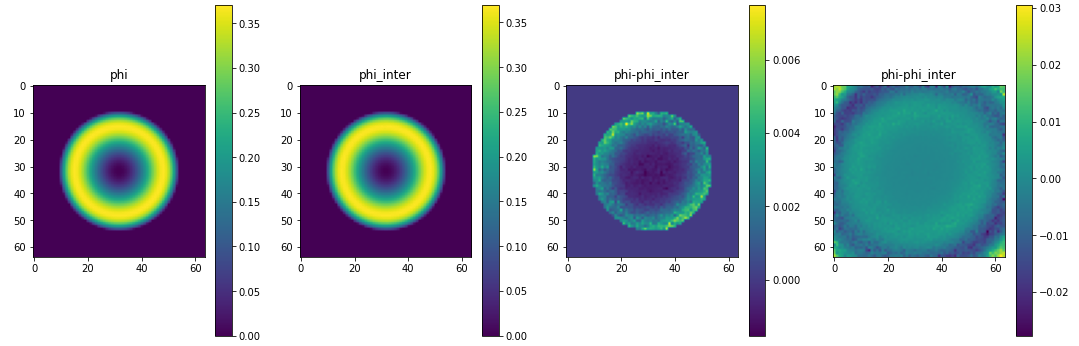
\includegraphics[width=0.9\linewidth]{results_griddata.png}
\end{minipage}

Il semblerait que sur le bord du cercle, les résultats soit moins bons. On a pas cherché à comprendre plus loin car on va utiliser la fonction extrapolate de FEniCS.


\subsubsection*{Extrapolate de FEniCS}

En milieu de semaine, on s'est rendu compte que le problème avec la foncion extrapolate que l'on avai eut la semaine dernière était que l'on pouvait n'incrémenter le degré d'interpolation que de 1.

\begin{minipage}{\linewidth}
	\centering
	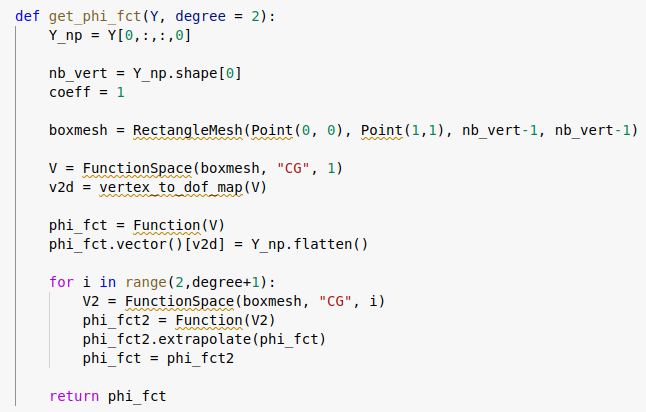
\includegraphics[width=0.5\linewidth]{get_phi_fct.png}
\end{minipage}

Voici les résultats obtenus pour une degré 2 :

\begin{minipage}{\linewidth}
	\centering
	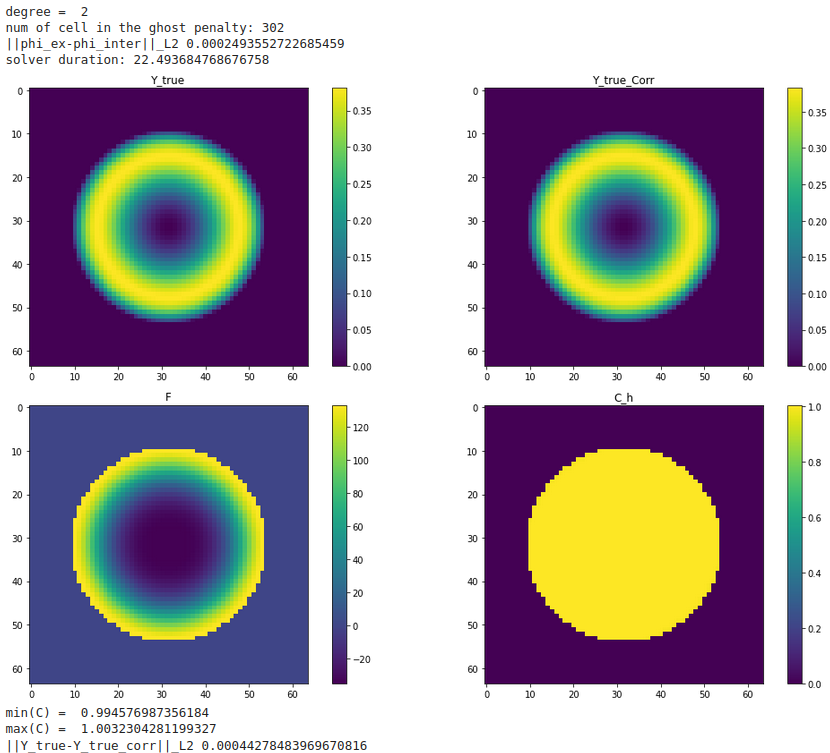
\includegraphics[width=0.9\linewidth]{results_extrapolate.png}
\end{minipage}


\conclusion{La semaine prochaine, on peut enfin entraîner le modèle car les installations ont été faites sur le nouveau pc.}
